\documentclass{bioinfo}
\copyrightyear{2012}
\pubyear{2012}
\raggedend
\setcounter{MaxMatrixCols}{24}
\usepackage{minted}
\usepackage{subfig}

\hyphenation{somito-genesis}

\begin{document}
\firstpage{1}

\title[Hes1 reaction-diffusion]{Reaction-diffusion simulation of a negative feedback inhibition system involving the \textit{Hes1} transcription factor}
\author[Standage]{Daniel S. Standage}
\address{Department of Genetics, Development, and Cell Biology, Iowa State University, Ames, IA 50011}

\history{May 1, 2012}

\maketitle

\section*{Background}

The Hes1 transcription factor plays a crucial role in eukaryotic development, regulating the morphological segmentation (\textit{somitogenesis}) in developing embryos.
Somitogenesis depends on carefully timed, periodic expression of a variety of Hes factors.
This expression pattern is established via a negative feedback inhibition system, in which the protein product of the Hes1 gene represses the transcription of that gene.
Consequently, Hes1 levels exhibit regular periodic oscillations throughout development, ensuring proper somitogenesis.

The Hes1 system is one of the best studied biological feedback inhibition systems \citep{Sturrock}.
For this project, I did a reaction-diffusion simulation of the Hes1 system.
A brief description is provided below.

\begin{figure}[h]
  \begin{center}
    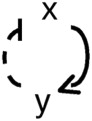
\includegraphics{../neg-fdbk-inh.jpg}
    \caption{The Hes1 system is a very simple and very well characterized feedback inhibition system. The mRNA (X) is used to produce protein (Y), which in turn inhibits the expression of more mRNA.}
  \end{center}
\end{figure}


\section*{Model}
For this project, I modeled the diffusion of Hes1 mRNA and protein from the nucleus to the cytoplasm.
For simplicity, the spatial component of the simulation was modeled in a single dimension, within the interval [-1, 1], with the nuclear membrane at 0.
The Hes1 system includes 2 biological species, but these were modeled mathematically as 4 species---nuclear and cytoplasmic variants of the mRNA and protein products.

The spatio-temporal evolution of these species was modeled using the following system of reaction-diffusion equations.
The $m$ symbol corresponds to mRNA, the $p$ symbol corresponds to protein, the $n$ subscript corresponds to nuclear species, the $c$ subscript corresponds to cytoplasmic species, and the $D$ symbol corresponds to diffusion rates.
\[ \frac{\delta[m_n]}{\delta t} = D_{m_n} \nabla^2[m_n] + \frac{\alpha_m}{1+([p_n]/\hat{p})^h} - \mu_m{m_n} \]
\[ \frac{\delta[m_c]}{\delta t} = D_{m_c} \nabla^2[m_c] - \mu_m{m_c} \]
\[ \frac{\delta[p_c]}{\delta t} = D_{p_c} \nabla^2[p_c] + \alpha_p[m_c] - \mu_p{p_c} \]
\[ \frac{\delta[p_n]}{\delta t} = D_{p_n} \nabla^2[p_n] - \mu_p{p_n} \]

\section*{Simulation}
The reaction-diffusion simulation was run using the MATLAB environment.
Source code for the simulation is included in the appendix.

The $\theta$ method which balances both the explicit and implicit approach to solving the system would be most appropriate for long-term simulations of this model.
However, for simplicity's sake my simulation used only the explicit approach.
I ran simulations for 2 different time intervals ([0,2] for 200 time steps and [0,20] for 2000 time steps) to see if I could reproduce oscillatory dynamics.

For 200 time steps, both the cytoplasmic species exhibited monotonic changes in concentration.
When simulated for 2000 time steps, the protein concentration did show a single oscillation, but definitely not multiple periodic oscillations.

\begin{figure}[t]
  \begin{center}
    \subfloat{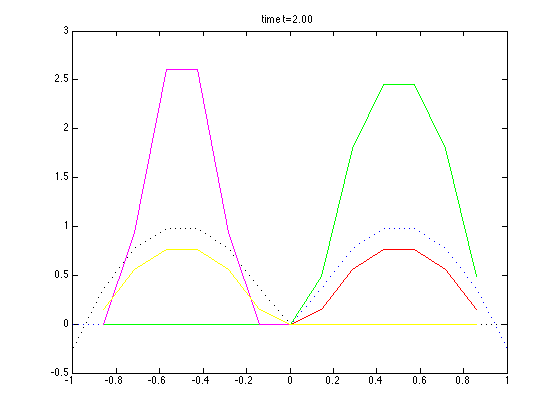
\includegraphics[width=200px]{../sim2.png}} \\
    \subfloat{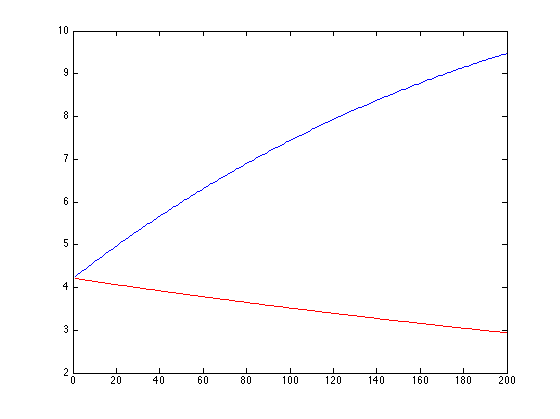
\includegraphics[width=200px]{../sim2t.png}} 
  \end{center}
  \caption{Simulation of the Hes1 system with 200 time steps. The top pane shows the concentration of all species across the spatial gradient, and the bottom pane shows the levels of protein (blue) and mRNA (red) in the cytoplasm over time.}
\end{figure}
\begin{figure}
  \begin{center}
    \subfloat{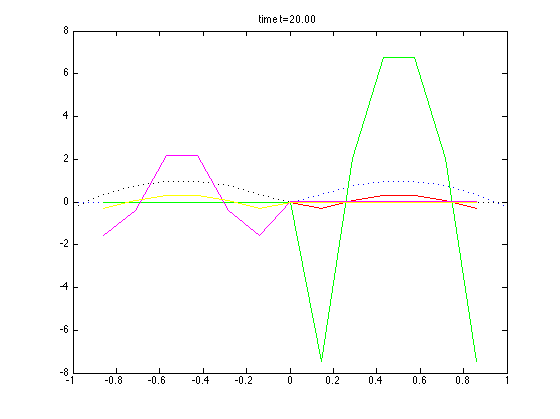
\includegraphics[width=200px]{../sim20.png}} \\
    \subfloat{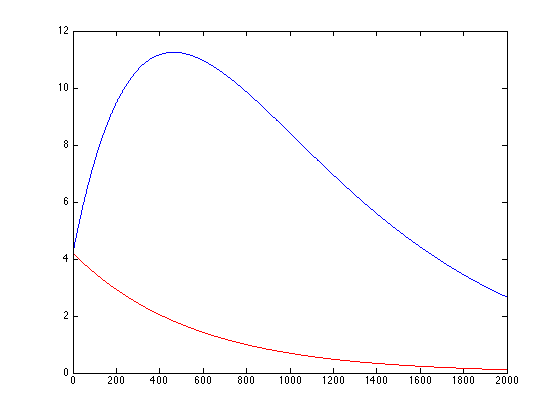
\includegraphics[width=200px]{../sim20t.png}} 
  \end{center}
  \caption{Simulation of the Hes1 system with 2000 time steps. The top pane shows the concentration of all species across the spatial gradient, and the bottom pane shows the levels of protein (blue) and mRNA (red) in the cytoplasm over time.}
\end{figure}

\section*{Discussion}
Unfortunately, it appears that my simulation was unable to recover the periodic oscillations of the Hes1 system.
I do not know whether this is due to an issue with my implementation or whether it is because I used an explicit approach to solving the system.

\section*{Acknowledgement}
I'd like to thank Tasos for his help and his patience, as well as Ali Berens and Srihari Radhakrishnan for their helpful discussions.


%\bibliographystyle{natbib}
%\bibliographystyle{achemnat}
%\bibliographystyle{plainnat}
%\bibliographystyle{abbrv}
%\bibliographystyle{bioinformatics}
%
%\bibliographystyle{plain}
%
%\bibliography{Document}


\begin{thebibliography}{}
\bibitem[Sturrock \textit{et~al}, 2011]{Sturrock} Marc Sturrock, Alan J. Terry, Dimitris P. Xirodimas, Alastair M. Thompson, and Mark A.J. Chaplain (2011) Spatio-temporal modelling of the Hes1 and p53-Mdm2 intracellular signalling pathways. \textit{Journal of Theoretical Biology}, \textbf{273}:15-31.

\end{thebibliography}

%\newpage
\onecolumn
\section*{Appendix: source code}
\begin{minted}[mathescape,
               linenos,
               numbersep=5pt,
               frame=lines,
               framesep=2mm]{matlab}
function simulate
% Daniel S. Standage
% May 1, 2012
% Adapted from code originally obtained from Benjamin Seibold at
% http://math.mit.edu/cse/codes/mit18086_fd_heateqn.m

% Parameters for Hes1 system
mu      = 3e-2;                % Degredation rate 
Df      = 7.5e-10;             % Diffusion coefficient
alpha_p = 1.11e-2;             % Translation rate
tr_i    = 2e-12;               % Transcription initiation rate

% Spatial dimension
n  = 13;                       % Number of internal grid points
x  = linspace(-1,1,n+2)';      % All grid points
xi = x(2:end-1);               % Internal (non-boundary) grid points
h  = x(2)-x(1);                % Discrete space interval
nm = ceil(n/2);                % First cytoplasmic grid point right of membrane

% Time dimension
dt = 1e-2;                     % Discrete time interval
tf = 2;                        % Final time

% Initialize vectors for nuclear and cytoplasmic variants of the mRNA and
% protein species
mn0 = g(x);                    % Nuclear mRNA
mn  = mn0(2:end-1);
pn0 = g(x);                    % Nuclear protein
pn  = pn0(2:end-1);   
mc0 = f(x);                    % Cytoplasmic mRNA
mc  = mc0(2:end-1);
pc0 = f(x);                    % Cytoplasmic protein
pc  = pc0(2:end-1);

I = eye(n);
R = diag(ones(1,n-1),1);

% M matrix for nuclear species
Dn = 2*I;
Dn(1,1) = 1;                   % Neumann boundary condition on left side
An =(R-Dn+R');
Mn = I-dt*mu+((Df*dt*An)/h^2); % Nuclear explicit time step
Mn(:,nm:end)=0;                % Nuclear membrane
Mn(nm:end,:)=0;

% M matrix for cytoplasmic species
Dc = 2*I;
Dc(end,end) = 1;                 % Neumann boundary condition on right side
Ac =(R-Dc+R');                              
Mc = I-dt*mu+((Df*dt*Ac)/h^2);   % Cytoplasmic explicit time step
Mc(:,1:nm)=0;                    % Nuclear membrane
Mc(1:nm,:)=0;

y_mn = zeros(1, ceil(tf/dt));
y_pn = zeros(1, ceil(tf/dt));
y_mc = zeros(1, ceil(tf/dt));
y_pc = zeros(1, ceil(tf/dt));

% Simulation
for tn = 1:ceil(tf/dt)
  %disp(sprintf('v=%dx%d, s=%dx%d\n', size(y_mn), size(mn)))
  mn = Mn*mn + tr_i.*(1+(pn/1e-2).^5); 
  pn = Mn*pn;
  pc = Mc*pc+alpha_p*mc;
  mc = Mc*mc;
  
  y_mn(tn) = sum(mn);
  y_pn(tn) = sum(pn);
  y_mc(tn) = sum(mc);
  y_pc(tn) = sum(pc);
  
  clf
  plot(x,mc0,'b:',x,mn0,'k:',xi,mc,'r.-',xi,pc,'g.-',xi,mn,'m.-',xi,pn,'y.-')
  title(sprintf('time t=%0.2f',tn*dt))
  drawnow
end

%clf
%plot(1:ceil(tf/dt), y_pc, 'b', 1:ceil(tf/dt), y_mc, 'r')

% Initial condition function for cytoplasmic species
function y = f(x)
y = zeros(size(x));
q = x > 0 ;
y(q) = 1-(5*(x(q)-0.5).^2);

% Initial condition function for nuclear species
function y = g(x)
y = zeros(size(x));
q = x < 0 ;
y(q) = 1-(5*(x(q)+0.5).^2);
\end{minted}

\end{document}
